% pic1
% equk,eqn
Eine ideale Spannungsquelle liefert eine konstante Spannung unabh�ngig von dem Strom, welcher ihr
entnommen wird. Im Gegensatz dazu stellt man fest, das eine reale Spannungsquelle sehr wohl von 
dem entnommenen Strom abh�ngt. Um dieses Verhalten vereinfacht darzustellen, stellt man sich die
reale Spannungsquelle als eine ideale Spannungsquelle mit der konstanten Spannung $U_0$, auch 
Leerlaufspannung gennant, in Reihe 
geschaltet mit einem Widerstand $R_i$ vor. So ist zu erkl�ren, dass bei entnommenem Strom die Klemmspannung
kleiner ist als die Leerlaufspannung. Wird der Verbraucher vereinfacht durch einen Widerstand $R_a$
dargestellt, so lassen sich aus den Kirchhoffschen Gesetzten folgende Beziehungen f�r die Klemmspannung
$U_k$ und die Leistung $N$ herleiten (vgl. Abb. \ref{pic1}).
\begin{align}
U_k&=I R_a=U_0 - I R_i \label{equk} \\
N&=I^2 R_a \label{eqn}
\end{align}
Kompliziertere Spannungsquellen wie elektrische Generatoren lassen sich teilweise auch �ber einen
Innenwiderstand darstellen, der nun aber eine differentielle Gr��e ist.
	\begin{figure}[h]
		\begin{center}
		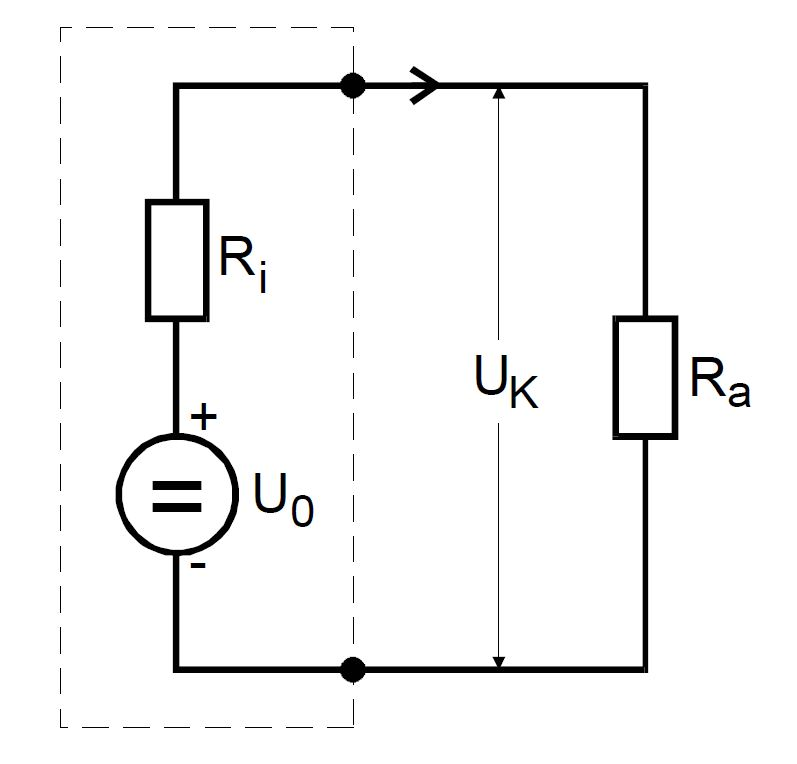
\includegraphics[scale=0.3]{pic1.jpg}
		\caption{Ersatzschaltbild einer realen Spannungsquelle [1]}
		\label{pic1}
		\end{center}	
	\end{figure}
\FloatBarrier


